\chapter{مقدمه}

\section{اهمیت مسیریابی بهینه در سیستم های حمل و نقل خودران}
توسعه سیستم‌های اتومات مانند هواپیماهای بدون سرنشین، وسایل نقلیه هدایت‌شونده خودکار و ربات‌های خودکار مزایای بسیاری را برای انسان داشته اند . توسعه وسایل نقلیه خودران منجر به افزایش ایمنی جاده ها و بهبود مصرف انرژی شده است. برای خودران سازی وسایل نقلیه باید نوعی سیستم داشت تا مسیرهای خود را مطابق با محیطی که قرار است در آن حرکت کنند برنامه ریزی کند. خواسته ی ما در این گونه مسائل این است که  این مسیرها تا حد امکان کوتاه باشند و وسیله نقلیه به راحتی حرکت کند و از همه مهمتر اینکه بدون مانع باشند .
با این حال، تحقیق در مورد برنامه ریزی حرکتی سیستم های خودران جدید نیست و به دهه 1950 برمی گردد، با الگوریتم هایی مانند جستجوی عرضی و جستجوی عمقی در مرحله اولیه تحقیقات برنامه ریزی حرکتی فرموله شده است. از آن زمان تاکنون چندین پیشرفت بزرگ در توسعه الگوریتم‌های برنامه‌ریزی حرکت صورت گرفته است . 
\cite{paliwal2023survey}

. یکی از الگوریتم های مهم برای هوشمندسازی و توانمد سازی این وسایل برای مسیریابی الگوریتم جست و جوی 
\lr{*A}
می باشد .هدف اصلی در
\cite{paliwal2023survey}
بر این است که انواع مختلفی از تغییرات این الگوریتم را در مسائل متفاوت برررسی نماید و آن ها را براساس زمان اجرا و برخی دیگر از ویژگی ها بررسی نماید .
\section{تاریخچه}
پیتر هارت 
\lr{(Peter Hart)}
، نیلز نیلسون 
\lr{(Nils Nilsson) }
و برترام رافائل 
\lr{(Bertram Raphael)} 
از موسسه پژوهشی استنفورد 
\lr{(Stanford Research Institute) }
که اکنون با عنوان اس‌آرآی اینترنشنال 
\footnote{\lr{SRI International}} 
فعالیت می‌کند، برای اولین‌بار، مقاله‌ای پیرامون الگوریتم
\lr{ *A }
را در سال ۱۹۶۳ منتشر کردند. این الگوریتم را می‌توان به عنوان افزونه‌ای از «الگوریتم دیکسترا» 
\footnote{\lr{ Dijkstra's Algorithm}}
در نظر گرفت که توسط «ادسخر دیکسترا»
\footnote{\lr{  Edsger Dijkstra}}
در سال ۱۹۵۹ ارائه شده است. الگوریتم 
\lr{*A}
با بهره‌گیری از «الگوریتم جستجوی کاشف» (جستجوی هیوریستیک  
\lr{Heuristics Search}) 
برای هدایت فرایند جستجو، به کارایی بهتری دست پیدا می‌کند
\cite{ELhamalgoritma_star}
.
\chapter{الگوریتم \lr{A*}}
\section{شیوه ی کار}
کاری که الگوریتم \lr{A*} انجام می‌دهد آن است که در هر گام، گره را متناسب با مقدار \lr{f}
که پارامتری مساوی با مجموع دو پارامتر دیگر \lr{g} و \lr{h} است انتخاب می‌کند. در هر گام، گره/خانه‌ای که دارای کمترین مقدار \lr{f}است را انتخاب و آن گره را پردازش می‌کند. \lr{g} و \lr{h} به روش ساده‌ای که در زیر بیان شده است محاسبه می‌شوند.
\begin{itemize}
	\item\lr{g}
	 هزینه حرکت از نقطه آغاز به یک مربع خاص در شبکه، با دنبال کردن مسیری که برای رسیدن به آن تولید شده است.
		\item\lr{h}
		 هزینه تخمین زده شده برای حرکت از یک خانه داده شده در شبکه به مقصد نهایی است. از \lr{h} معمولا با عنوان هیوریستیک یاد می‌شود. هیوریستیک چیزی به جز نوعی حدس هوشمندانه نیست. کاربر واقعا فاصله واقعی را تا هنگام یافتن مسیر نمی‌داند، زیرا هر مانعی (دیوار، آب و سایر موانع) ممکن است در مسیر باشد. راه‌های زیادی برای محاسبه \lr{h} وجود دارد به عنوان مثال فاصله ی مستقیم اقلیدسی یک ز مواردی است که می تواند در ماسئل به عنوان این حدس اولیه در نظر گرفته شود .

\end{itemize}
الگوریتم 
\lr{A*}
به نحوی الگوریتم دایکسترا است که راس ها را با اولویت 
$f(n)=g(n)+h(n)$
انتخاب می کند .
\begin{figure}[h]
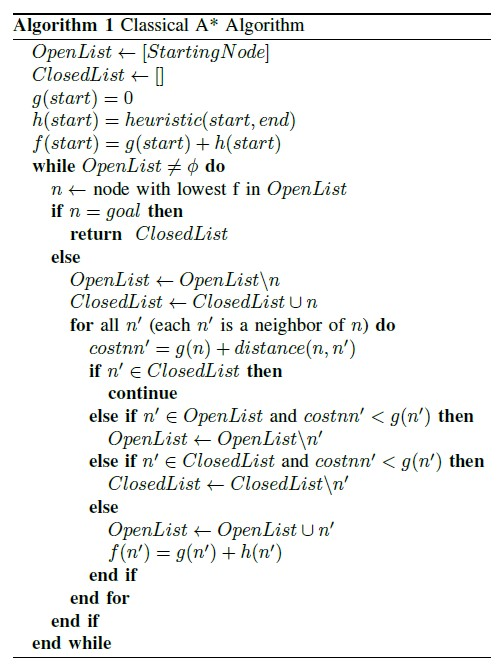
\includegraphics[scale=1]{code}
\centering
\caption{ شبه کد مربوط به الگوریتم \lr{A*}}
\cite{paliwal2023survey}
\label{improved}
\end{figure}

\chapter{دگرگونی های الگوریتم \lr{A*}}
\section{ورژن ها}
این الگوریتم به شیوه های متفاوت متناسب با شرایط فضای مسئله گسترش یافته است . در ادامه به برخی از این ورژن ها می پردازیم :






